% ====================================================================
%+
% SECTION:
%    section-name.tex  % eg lenstimedelays.tex
%
% CHAPTER:
%    chapter.tex  % eg cosmology.tex
%
% ELEVATOR PITCH:
%    Explain in a few sentences what the relevant discovery or
%    measurement is going to be discussed, and what will be important
%    about it. This is for the browsing reader to get a quick feel
%    for what this section is about.
%
% COMMENTS:
%
%
% BUGS:
%
%
% AUTHORS:
%    Phil Marshall (@drphilmarshall)  - put your name and GitHub username here!
%-
% ====================================================================

\section{Gravitational Wave Sources}
\def\secname{gw}\label{sec:\secname}


\credit{raffaellamargutti}, 
\credit{Doctor},
\credit{Fong},
\credit{Haiman},
\credit{Kalogera},
\credit{Trimble},
\credit{Zauderer}
%\noindent{\it Raffaella Margutti, Z. Doctor, W. Fong, Z. Haiman, V. Kalogera, V. Trimble, B.~A. Zauderer } % (Writing team)

% This individual section will need to describe the particular
% discoveries and measurements that are being targeted in this section's
% science case. It will be helpful to think of a ``science case" as a
% ``science project" that the authors {\it actually plan to do}. Then,
% the sections can follow the tried and tested format of an observing
% proposal: a brief description of the investigation, with references,
% followed by a technical feasibility piece. This latter part will need
% to be quantified using the MAF framework, via a set of metrics that
% need to be computed for any given observing strategy to quantify its
% impact on the described science case. Ideally, these metrics would be
% combined in a well-motivated figure of merit. The section can conclude
% with a discussion of any risks that have been identified, and how
% these could be mitigated.

The first detection of Gravitational Waves (GW) by the advanced LIGO/Virgo collaboration \citep{Abbott16, Abbott09, Acernese08} has recently opened a new window of exploration into our Universe. The amount of information that can be revealed by the properties of the GW emission is immense and holds promises for revolutionary insights, including accurate masses and spins of neutron stars and black holes, tests of General Relativity and an accurate census of the neutron star (NS) and black hole (BH) populations that might challenge our current understanding of massive stellar evolution. However, GW events are poorly localized (10-100 deg$^2$ at the time of LSST operations). The identification of EM counterparts would provide precise localization and distance measurements, in addition to the necessary astrophysical context (e.g. host galaxy properties, connection to specific stellar populations) to fully exploit the revolutionary power of this new GW era.


% --------------------------------------------------------------------

\subsection{Target measurements and discoveries}
\label{sec:\secname:targets}

The first GW event was found to be associated with the merger of two black holes \citep{Abbott16,Abbott16b}. Although no EM counterpart was expected to accompany a black-hole black-hole (BBH) merger, it seems now possible that even BBH mergers  might produce short GRB-like EM emission \citep{Connaughton16, Loeb16,Zhang16,Perna16,Stone16}. Indeed, in analogy with supermassive BH mergers, shocks might develop in the just-formed circumbinary accretion disk (if a disk forms), which can produce a bright afterglow following the BBH merger (e.g. \citealt{Lippai08,Corrales10,Schnittman13}). Albeit speculative in nature, it is advisable to keep an open mind about the possibility of EM counterparts to BBH mergers. 

The most promising and better understood EM counterparts to GW events are ``kilonovae" \citep{Li98, Metzger10, Metzger12,Kasen13,Barnes13}. Kilonovae are short-lived (typical time scale of one week), apparently faint ($z\sim21$ mag at peak at 120 Mpc), red ($i-z\approx1$ mag), isotropic transients (Fig. \ref{Fig:kilonova}) due to the radioactive decay of r-process elements synthesized in the merger ejecta of a NS-NS or NS-BH system. These merging systems are the favored progenitors of short GRBs. Indeed, the signature of a kilonova emission has been recently found following the short GRB\,130603B \citep{Berger13,Tanvir13}. The key piece of information that enabled the discovery of kilonova-like emission associated with  this short GRB was its sub-arcsecond localization enabled by the detection of the optical afterglow, which allowed for an effective kilonova search with the Hubble Space Telescope (Fig. \ref{Fig:kilonova}). In contrast, the typical localization region of GW events in the LSST era is expected to be of the order of a few tens of square degrees \citep{aaa+13}. It is thus clear that the major challenges faced by the optical follow-up of GW events is represented by the combination of poor localizations with faint and fast evolving red electromagnetic counterparts.

The detection of an optical counterpart in conjunction with a GW event will significantly leverage the GW signal.
LSST, with its the wide FOV, wavelength coverage and exquisite sensitivity is uniquely poised to identify and characterize counterparts to GW events. 

\begin{figure}
\vskip -0.0 true cm
\centering
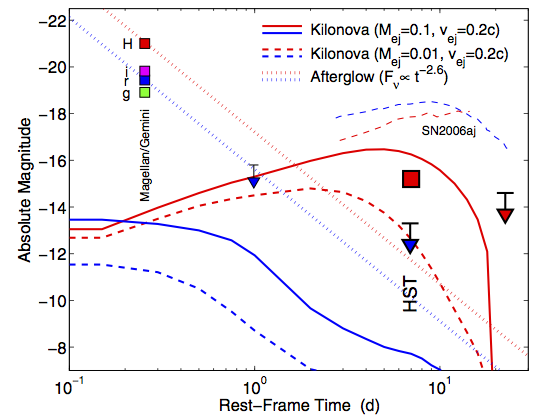
\includegraphics[scale=0.85]{figs/transients/kilonovaBerger.png}
\caption{Kilonova signature in the short GRB\,130603B as revealed by the Hubble Space Telescope (HST). The Magellan and Gemini telescopes sampled the optical afterglow of the GRB (dotted lines). The kilonova light starts to dominate the emission in the H band around a few days after the merger. Thick and dashed lines: theoretical kilonova models from \cite{Barnes13} showing that kilonovae are fast-evolving, faint and red transients. The light-curve of the SN\,2006aj associated with the long GRB\,060218  is also shown for comparison. From \cite{Berger13}.}
\label{Fig:kilonova}
\end{figure}


% --------------------------------------------------------------------



% --------------------------------------------------------------------

\subsection{OpSim Analysis and Discussion}
\label{sec:\secname:analysis}

Effective follow up of GW triggers relies on the capability to sample a relatively large portion of the sky, repeatedly, over a time scale $<1$ week, with different filters \citep{Cowperthwaite15}. In the optical band, the kilonova signature is expected to be more prominent in the $i$, $z$  and $y$ filters, which we identify as the most promising filters for the kilonova search. We emphasize however that another set of contemporaneous observations in  a ``bluer" filter is necessary to acquire color information and distinguish kilonovae from other fast-evolving transients.

We use the median inter-night gap  for visits in the same filter derived from the candidate Baseline Cadence \texttt{minion\_1016} to show that, in the absence of a Target of Opportunity (ToO) capability, it is \emph{not} possible for LSST  to play a major role in the identification of EM counterparts of GW triggers.  

To identify kilonova candidates we need at least 2 observations acquired within $\sim 1$ week  of the GW event \citep{Cowperthwaite15}.
Using the inter-night gap distribution for visits in the $y$ filter (which is the most promising filter for a kilonova search), the area of the sky covered with cadence  $\Delta t<7$ days at any given time, is $A_{sky}\sim 3000$ deg$^2$ (including deep drilling fields).  This is the area that can be searched for fast evolving transients.  Two important considerations follow:

\begin{itemize}
\item[(1)] $A_{sky}$ only covers $P\sim7$\% of the sky. The  probability that the \emph{entire} GW localization region is contained, by chance,  within $A_{sky}$ is thus very small.
\item[(2)] Even if LSST is able to cover a meaningful portion of the GW region, we would still not have color information, and we would thus be unable to filter out contaminating transients.
\end{itemize}

\textbf{We conclude that relying on the serendipitous alignment of the LSST fields with the GW localization map is not an effective strategy to follow up GW triggers and identify their EM counterparts. We thus strongly recommend a ToO capability as part of the baseline LSST operations strategy.}

Ideally, the ToO capability will allow for imaging of the GW localization map at least twice over $\Delta t\lesssim$1 week with a ``red" filter ($i$, $z$  or $y$),  and  will include the possibility to designate a desired set of filters to obtain color information. By the time of LSST operation the typical size of the GW localization region is expected to be 10-100 deg$^2$, which would require a small number of LSST re-pointings. We thus do \emph{not} anticipate a significantly disruptive impact on other LSST campaigns (especially if only the GW triggers with the best localizations in the southern sky are selected for LSST ToOs).

\textbf{At the price of re-shuffling a reasonably small number of fields, \emph{if} equipped with ToO capabilities, LSST can be the premier player in the era of EM follow up to GW sources.}






% ====================================================================

\navigationbar
